%Sección
\section{Minería de Datos}
\lhead[\thepage]{\thesection Minería de Datos}
También conocida como "Descubrimiento de conocimiento en bases de datos" (KDD por sus siglas en ingles). Se define generalmente como el proceso por el cual se descubren patrones o conocimiento relevante en fuentes de datos, p.ej., base de datos, textos, imágenes, la Web, etc. Dichos patrones deben ser validos, potencialmente útiles, y comprensibles.La minería de datos es un campo multidisciplinario que involucra  estadísticas,\emph{ machine learning}, inteligencia artificial, bases de datos, recuperación de la información, y visualización.\cite{webmining}

Son muchas las tareas involucradas en este proceso. Entre las mas comunes se tiene la clasificación, clusterización, minería por reglas de asociación, y minería por patrones secuenciales.\cite{webmining}



%--------
% Etapas del proceso KDD

% El proceso de creación de un modelo en minería de datos es un proceso cíclico, dinámico e interactivo, por lo tanto, es posible que se repita en varias ocasiones hasta obtener el modelo adecuado, sus fases suelen ser:

% 1. Definición del problema y selección del conjunto de datos: Consiste en definir el problema y los objetivos del proyecto 55. Se organiza la información disponible y la fuente de las mismas, se definen las variables objetivas e independientes y se seleccionan los registros que se encuentran disponibles para ser empleados.

% 2. Análisis de las propiedades de los datos: Consiste en explorar y revisar los datos disponibles, para luego definirlos, evaluar el valor correspondiente y verificar si están bien captados o no.

% 3. Transformación, preparación o pre procesamiento de datos: Los datos obtenidos pueden hallarse dispersos o bien estar almacenados en diversos formatos, así mismo, pueden darse casos de valores perdidos (valores incorrectos o ausentes), en esta etapa se busca depurar la base de datos eliminando aquellos que no resultan válidos, generando los faltantes y buscando correlaciones ocultas entre ellos, para de esta forma generar una estructura final compuesta de datos adecuados y precisos que faciliten su transformación y posterior análisis.

% 4. Generar modelos: Consiste en la definición de los algoritmos y técnicas de minería de datos que se van a emplear en el tratamiento de los datos, se busca obtener patrones que representen un conocimiento útil y de valor. Dichos patrones son obtenidos a través de un proceso conocido como entrenamiento, este consiste en aplicar un algoritmo a una estructura de datos para obtener patrones de ella, por tanto, dichos patrones variarán en función de los datos y el algoritmo empelado 55. Cabe acotar que en caso de que los datos cambien, será necesario cambiar el proceso de minería empleado.

% 5. Explorar y validar modelos: Consiste en la interpretación de los resultados obtenidos para determinar si las conclusiones resultan válidas y satisfactorias. En caso de que ninguno de los modelos generados funcione, el proceso puede repetirse desde el inicio o desde un paso anterior.

% 6. Implementar y actualizar modelos: En esta fase se colocan en uso los modelos que funcionen mejor para incorporarlo a los sistemas de análisis de información de la organización, dichos modelos permitirán luego generar información de utilidad para tomar decisiones de negocio.

%------------------------------------------------------
% descomentar >>>
\subsection{El proceso de la Minería de Datos}
Según \cite{webmining} una aplicación de minería de datos usualmente comienza con el entendimiento del dominio del problema por los analistas de datos, quienes luego identifican fuentes de datos adecuadas y los datos objetivo. Una vez que se obtienen los datos se comienza el proceso de minería, este generalmente se lleva acabo en 3 pasos: 
\begin{itemize}
\item Pre-procesamiento: Los datos crudos (obtenidos de la fuente sin previo procesamiento) son limpiados de ruidos y anormalidades. En muchos casos también es necesaria la reducción de estos a través de muestreo y selección de atributos o características.
\item Minería de datos: Los datos procesados son pasados a un algoritmo encargado de producir los patrones o conocimiento.
\item Post-procesamiento: En muchos casos, no todos los patrones descubiertos son útiles. Este paso identifica aquellos que tienen un valor para su aplicación. Varias evaluaciones y técnicas de visualización son utilizadas para hacer esta decisión. 
\end{itemize}

Este proceso es iterativo la mayoría de las veces . Usualmente conlleva varias rondas para alcanzar un resultado final satisfactorio, que es luego incorporado en una tarea operacional del mundo real. \cite{webmining}

\subsection{Tipos de modelo}

Los métodos y algoritmos aplicables en la minería de datos son variados, estos se definen en función de la elección del problema de estudio y los datos disponibles. A grandes rasgos, es posible identificar dos tipos de modelos:

\subsubsection{Modelos predictivos}

Como su nombre lo indica, están asociados a tareas que implican predicción, predicen el valor de un atributo o variable de interés basado en el valor de otros atributos. Dentro de este modelo, se encuentran los algoritmos de aprendizaje supervisados, en los cuales el proceso de modelaje es realizado sobre un conjunto de ejemplos formados por entradas al sistema y la respuesta que se debería dar ante cada una de ellas, de esta forma, el modelo es entrenado a través de datos para predecir una variable basada en dichos datos \cite{54}. Los modelos predictivos pueden ser de dos tipos:
 \begin{itemize}
 \item Clasificación: Dada una cantidad de registros que contienen una serie de atributos, se examinan las características de dicho registro y se le asigna una clase o categoría lo más exacta posible. En este tipo de modelos se incluyen las redes neuronales, los árboles de decisiones y el análisis discriminante.
 \item Regresión: Dada una colección de registro, se intenta predecir un valor futuro (Lo más exactamente posible) tomando como base un conjunto de valores pasados. Este modelo incluye series temporales, técnicas bayesianas, análisis de varianza y covarianza, etc.
 \end{itemize}

\subsubsection{Modelos descriptivos}

Como su nombre lo indica, se asocian a tareas descriptivas, es decir, identifican patrones o tendencias que explican o describen los datos y sus propiedades, sin tener conocimiento previo acerca de los patrones buscados. A esta categoría pertenecen los algoritmos de aprendizaje no supervisados, en donde la respuesta no está dada, sino que el proceso de modelaje se lleva a cabo únicamente sobre un registro de entradas, a partir de las cuales el sistema debe reconocer patrones para etiquetar nuevas entradas. Los modelos descriptivos pueden ser de tres tipos:

\begin{itemize}
\item Agrupación/Clustering/Segmentación: Dada una colección de registros con distintos atributos, se pretenden hallar grupos con características muy similares entre sí pero muy diferentes con respecto a los otros. No dependen de clases predefinidas.
\item Análisis de asociación: Dada una colección de registros, se busca descubrir patrones fuertemente asociados con los datos, es decir, combinaciones de atributos frecuentes que permitan establecer reglas de asociación.
\item Búsqueda de secuencias y detección de anomalías: Dada una colección de registros con una serie de atributos, se busca identificar aquellos registros cuyas características sean significativamente diferentes del resto. Este método suele ser empleado para analizar series de tiempo y detectar desviaciones significativas del comportamiento normal.
\end{itemize}

\subsection{Mineria Web}
La mineria web (\emph{Web mining}), hace referencia a la minería de datos aplicada sobre la web, su meta es la de encontrar información útil o conocimiento de la estructura de enlaces web, contenido de las paginas y uso de los datos. A diferencia de la minería de datos tradicional donde generalmente se trabaja con datos estructurados y estructuras relacionales por naturaleza, un aspecto esencial de la minería de datos web es el tener que lidiar con datos no estructurados.\cite{webmining,minwebSoumen}

Una característica que distingue a la web es la formación espontanea y evolución de clusters inducidos por tópicos y comunidades inducidas por enlaces en el grafo web. La existencia de los enlaces añaden una cantidad importante de información mas allá de la búsqueda de texto, organización por relevancia, clasificación y clusterizacion. Otra característica es que paginas HTML bien formadas representan una estructura de árbol, con texto y atributos en los nodos, esto puede revelar pistas importantes para algoritmos de minería de contenido.\cite{minwebSoumen}

Según Bing Liu (2011) las tareas de minería web pueden subdividirse basándose en el tipo de datos usados en el proceso de minería:
\begin{itemize}
\item Minería de la estructura web: descubre conocimiento útil de los enlaces (\emph{hyperlinks}) que representan la estructura de la web. Por ejemplo, de los enlaces, se pueden descubrir comunidades de usuarios que comparten un interés mutuo.
\item Minería del contenido web: extrae información útil o conocimiento del contenido de paginas web. Se puede clasificar y clusterizar paginas web en base a su tópico. En este aspecto es muy similar a la minería de datos tradicional. Sin embargo, es también posible descubrir patrones en paginas web para extraer datos útiles en base a la interacciones que tienen los usuarios con dichas paginas, como foros, redes sociales,  . Tareas que no son parte de la minería de datos tradicional.
\item Minería del uso web: se refiere al descubrimiento de patrones de acceso a las web por parte del usuario, el proceso de minería se aplica sobre web logs donde se almacena todas las acciones que lleva a cabo el usuario.
\end{itemize}

\subsection{Web Crawling y Web Scraping}

En \cite{crawlingwebCho} se define un web crawler como un programa de gran escala que recolecta decenas de miles de paginas web por segundo. Generalmente para luego almacenarlas en un repositorio local e indexarlas en base a palabras claves. Concepto similar se tiene en \cite{crawlingwebPant} donde los web crawlers se definen como programas que explotan la estructura en grafo de la web para moverse de pagina en pagina,su motivación principal es la de recuperar las paginas web y añadirlas a un repositorio local, para luego ser usadas a conveniencia por el programa.

Uno de los puntos claves para la definición de lo que es un web crawler es su capacidad para moverse en la web a través de enlaces. Y marca una diferencia importante con el concepto de Web Scraping. 

Web Scraping es el termino acuñado para la extracción de datos de una pagina web previamente encontrada por un web crawler.\cite{webscrapLawson}

\subsubsection{Infraestructura de Web Crawling}
\emph{Crawling} puede ser visto como un problema de búsqueda en un grafo. La Web es vista como un grafo de grandes proporciones con paginas como sus nodos y enlaces como sus vértices. Un \emph{crawler} empieza en alguno de los nodos del grafo (semillas) y luego sigue los vértices para alcanzar otros nodos. El proceso de obtener una pagina y extraer los enlaces es análogo a expandir un nodo en búsqueda de grafos. Un \emph{crawler} por tópico trata de seguir los vértices de los que se espera lleven a porciones del grafo que son relevantes a un tópico.\cite{crawlingwebPant} 

\begin{figure}[!htbp]
    \centering
    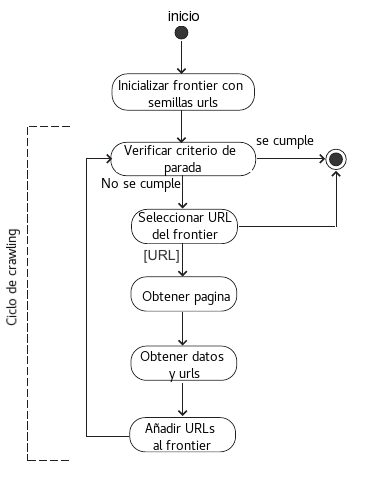
\includegraphics[width=0.5\textwidth]{Figuras/basic_sequential_crawler.png}
    \caption{Crawler basico secuencial}
    \label{fig:basiccrawler}
    \source{Imagen extraída de \cite{crawlingwebPant}}
\end{figure}


En la Figura \ref{fig:basiccrawler} se muestra el flujo básico de un \emph {crawler} secuencial. El \emph{crawler} mantiene una lista de URLs sin visitar llamada \emph{frontier}. Dicha lista es inicializada con semillas URLs (termino acuñada para referirse a URLs que inicial el proceso de \emph{crawling}). Cada iteración de \emph{crawling} involucra tomar la siguiente URL a explorar del \emph{frontier}, obtener la pagina que corresponde a la URL a traves de HTTP, extraer de esta pagina las URLs e información requerida (se podría considerar como el proceso de Webscraping), y finalmente agregar las URLs no visitadas al \emph{frontier}.

Los URLs son asignados al \emph{frontier} basándose en un puntaje previo que representa un estimado del beneficio de visitar dicha pagina.El proceso de \emph{crawling} termina cuando un numero especifico de paginas han sido exploradas. Si el \emph{frontier} esta vacío, el proceso termina de forma automática.\cite{crawlingwebPant} 